% Trying to break the document up a bit.  This command simply inserts the contents of the file at this point.  It contains the document license, preamble, and title page: things that aren't likely to change more than once.  This can be used to separate discrete parts of a document into files that are easier to edit at one time.
%%%%%%%%%%%%%%%%%%%%%%%%%%%%%%%%%%%%%%%%%%%%%%%%%%%%%%%%%%%%%%%%%%%%%%
% This layout was adapted from one found at latextemplates.com which
% was adapted from another.
%
% License: CC BY-NC-SA 3.0
% (http://creativecommons.org/licenses/by-nc-sa/3.0/)
%
% Original header:
%
% This is a LaTeX version of the sample laboratory report from
% Virginia Tech's copyrighted 08-09 CHEM 1045/1046 lab manual.
% Reproduction of this one appendix section for academic purposes
% should fall under fair use.
%
%%%%%%%%%%%%%%%%%%%%%%%%%%%%%%%%%%%%%%%%%%%%%%%%%%%%%%%%%%%%%%%%%%%%%%

\documentclass{article}

\usepackage{graphicx}
% \usepackage[acronym]{glossaries} % Lets us use acronyms
\usepackage{multicol}
\usepackage{amsmath}
\usepackage{siunitx} % SI units in math mode
\usepackage{subcaption}

\author{}
\title{ELEC-313 \\ Lab 5: CMOS Circuits\\ }
\date{\today}

% \loadglsentries{acronyms} % Actually loads 'acronyms.tex'
% \makeglossaries

\begin{document}

\maketitle

\begin{center}
  \begin{tabular}{lr}
    Date Performed: & October 16, 2013 \\
    Partners:       & Charles Pittman    \\
    & Stephen Wilson     \\
  \end{tabular}
\end{center}

\newpage

\tableofcontents
\listoffigures
\listoftables
\newpage

% Number the enumerate environment (unordered lists) by letter:
\renewcommand{\labelenumi}{\alph{enumi}.}

\section{Objective}
\label{sec:objective}

The objective is to construct and observe the operation of a CMOS inverter and NAND gate.

\section{Equipment}
\label{sec:equipment}

\begin{tabular}{ll}
  \centering
  Transistor: 1N4007 & Power supply: HP E3631A \\
  Resistors: \SI{330}{\ohm} (x3), \SI{2.2}{\kilo\ohm}, \SI{33}{\kilo\ohm} & Multimeters: Fluke 8010A (x2) \\
\end{tabular}

\section{Schematics}
\label{sec:schematics}

\begin{figure}[hbtp]
  \centering
  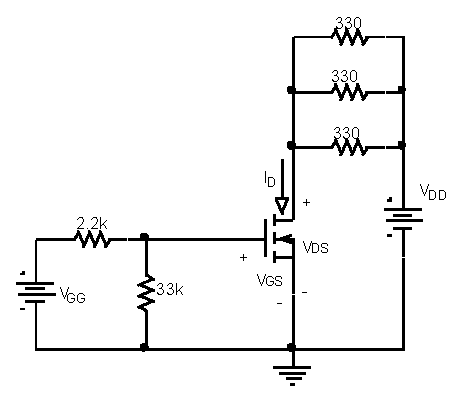
\includegraphics[width=0.6\textwidth]{circuit}
  \caption{\label{fig:circuit} Circuit used in this lab.}
\end{figure}

% \begin{figure}[hbtp]
%   \centering
%   \begin{subfigure}[b]{0.4\textwidth}
%     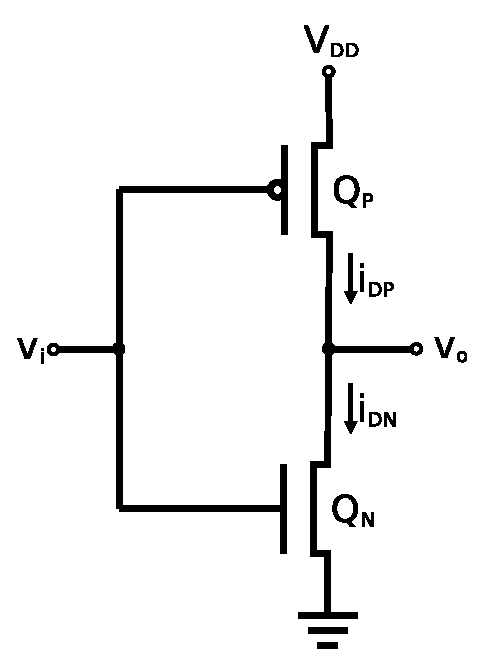
\includegraphics[width=\textwidth]{invert}
%     \caption{\label{schem:inverter} CMOS Inverter}
%   \end{subfigure}%
%   ~
%   \begin{subfigure}[b]{0.4\textwidth}
%     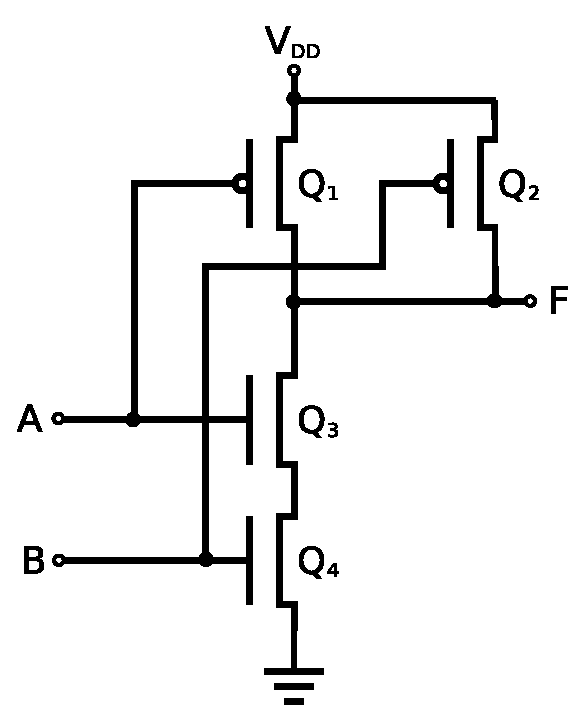
\includegraphics[width=\textwidth]{nand}
%     \caption{\label{schem:nand} CMOS NAND}
%   \end{subfigure}
%   \caption{\label{fig:schematics} Circuits used in this lab.}
% \end{figure}

\section{Procedure}
\label{sec:procedure}

\subsection{DC Characteristics}
\label{sec:inverter}

\begin{enumerate}
\item Obtain the 2N7000 MOSFET transistor and resistors needed to build the circuit shown.
\item Construct the circuit of figure 2. Use the HP multi-meter to measure the drain current, $I_D$ , and the Fluke multi-meters to measure $V_{DS}$ and $V_{GS}$. Use the +6 V power supply for $V_{GG}$ and the +25 V supply for $V_{DD}$.
\item Set $V_{GG}$ to 0 V and $V_{DD}$ to 5 V and measure $V_{DS}$ and $I_D$.
 \item Slowly increase $V_{GG}$ until the transistor just begins to conduct current as evidenced by a small drop in $V_{DS}$. Record the value of $V_{GS}$ as the Gate Threshold Voltage, $V_{TN}$.
\item Adjust $V_{GG}$ to increase $V_{GS}$ by 0.2 V above the threshold. Readjust $V_{DD}$ to return $V_{DS}$ to 5 V, and then measure the drain current ($I_D$ ). Record the value of $V_{GS}$ in the first column of table1, and record the value of $I_D$ in the second column (the $V_{DS}$ = 5 V column).
\item Continue to increase $V_{GS}$ in steps of 0.2 V while maintaining $V_{DS}$ at 5 V. Measure the drain current at each step. Record the values of $V_{GS}$ and $I_D$ in table 1. Stop this process when the drain current reaches approximately 80mA.
\item Complete the entries in table 1 by adjusting $V_{DD}$ and $V_{GG}$ to obtain the various required $V_{DS}$ and $V_{GS}$ values, then measuring $I_D$ at each value. Do not exceed 80mA drain current.
\end{enumerate}

\subsection{Small-Signal Transconductance}
\label{sec:nand}

\begin{enumerate}
\item Adjust $V_{GG}$ and $V_{DD}$ to obtain $V_{DS}$ = 5 V and $I_D$ = 10 mA.
\item Record the value of $V_{GS}$ as $V_{G1}$.
\item Record the exact measured value of $I_D$ and assign it to $I_{D1}$. Use the full resolution of the HP multimeter.
\item Increase $V_{GS}$ by 10 mV and record it value as $V_{G2}$.
\item Measure $I_D$ , recording it as $I_{D2}$.
\item Compute the small signal transconductance (Eq~\ref{eq:transconduct}).
\end{enumerate}

\section{Results}
\label{sec:results}

The following table shows several $V_{GS}$ values that are just slightly over the overdrive voltage $V_{OV}$ and gives an idea of the amount of variation for values resulting from equation 2.

\begin{figure}[hbtp]
  \centering
  \resizebox{1.0\textwidth}{!}{% GNUPLOT: LaTeX picture with Postscript
\begingroup
  \makeatletter
  \providecommand\color[2][]{%
    \GenericError{(gnuplot) \space\space\space\@spaces}{%
      Package color not loaded in conjunction with
      terminal option `colourtext'%
    }{See the gnuplot documentation for explanation.%
    }{Either use 'blacktext' in gnuplot or load the package
      color.sty in LaTeX.}%
    \renewcommand\color[2][]{}%
  }%
  \providecommand\includegraphics[2][]{%
    \GenericError{(gnuplot) \space\space\space\@spaces}{%
      Package graphicx or graphics not loaded%
    }{See the gnuplot documentation for explanation.%
    }{The gnuplot epslatex terminal needs graphicx.sty or graphics.sty.}%
    \renewcommand\includegraphics[2][]{}%
  }%
  \providecommand\rotatebox[2]{#2}%
  \@ifundefined{ifGPcolor}{%
    \newif\ifGPcolor
    \GPcolortrue
  }{}%
  \@ifundefined{ifGPblacktext}{%
    \newif\ifGPblacktext
    \GPblacktextfalse
  }{}%
  % define a \g@addto@macro without @ in the name:
  \let\gplgaddtomacro\g@addto@macro
  % define empty templates for all commands taking text:
  \gdef\gplbacktext{}%
  \gdef\gplfronttext{}%
  \makeatother
  \ifGPblacktext
    % no textcolor at all
    \def\colorrgb#1{}%
    \def\colorgray#1{}%
  \else
    % gray or color?
    \ifGPcolor
      \def\colorrgb#1{\color[rgb]{#1}}%
      \def\colorgray#1{\color[gray]{#1}}%
      \expandafter\def\csname LTw\endcsname{\color{white}}%
      \expandafter\def\csname LTb\endcsname{\color{black}}%
      \expandafter\def\csname LTa\endcsname{\color{black}}%
      \expandafter\def\csname LT0\endcsname{\color[rgb]{1,0,0}}%
      \expandafter\def\csname LT1\endcsname{\color[rgb]{0,1,0}}%
      \expandafter\def\csname LT2\endcsname{\color[rgb]{0,0,1}}%
      \expandafter\def\csname LT3\endcsname{\color[rgb]{1,0,1}}%
      \expandafter\def\csname LT4\endcsname{\color[rgb]{0,1,1}}%
      \expandafter\def\csname LT5\endcsname{\color[rgb]{1,1,0}}%
      \expandafter\def\csname LT6\endcsname{\color[rgb]{0,0,0}}%
      \expandafter\def\csname LT7\endcsname{\color[rgb]{1,0.3,0}}%
      \expandafter\def\csname LT8\endcsname{\color[rgb]{0.5,0.5,0.5}}%
    \else
      % gray
      \def\colorrgb#1{\color{black}}%
      \def\colorgray#1{\color[gray]{#1}}%
      \expandafter\def\csname LTw\endcsname{\color{white}}%
      \expandafter\def\csname LTb\endcsname{\color{black}}%
      \expandafter\def\csname LTa\endcsname{\color{black}}%
      \expandafter\def\csname LT0\endcsname{\color{black}}%
      \expandafter\def\csname LT1\endcsname{\color{black}}%
      \expandafter\def\csname LT2\endcsname{\color{black}}%
      \expandafter\def\csname LT3\endcsname{\color{black}}%
      \expandafter\def\csname LT4\endcsname{\color{black}}%
      \expandafter\def\csname LT5\endcsname{\color{black}}%
      \expandafter\def\csname LT6\endcsname{\color{black}}%
      \expandafter\def\csname LT7\endcsname{\color{black}}%
      \expandafter\def\csname LT8\endcsname{\color{black}}%
    \fi
  \fi
  \setlength{\unitlength}{0.0500bp}%
  \begin{picture}(7200.00,5040.00)%
    \gplgaddtomacro\gplbacktext{%
      \csname LTb\endcsname%
      \put(726,440){\makebox(0,0)[r]{\strut{}0mA}}%
      \csname LTb\endcsname%
      \put(726,1307){\makebox(0,0)[r]{\strut{}5mA}}%
      \csname LTb\endcsname%
      \put(726,2174){\makebox(0,0)[r]{\strut{}10mA}}%
      \csname LTb\endcsname%
      \put(726,3041){\makebox(0,0)[r]{\strut{}15mA}}%
      \csname LTb\endcsname%
      \put(726,3908){\makebox(0,0)[r]{\strut{}20mA}}%
      \csname LTb\endcsname%
      \put(726,4775){\makebox(0,0)[r]{\strut{}25mA}}%
      \csname LTb\endcsname%
      \put(858,220){\makebox(0,0){\strut{}0 V}}%
      \csname LTb\endcsname%
      \put(1453,220){\makebox(0,0){\strut{}2 V}}%
      \csname LTb\endcsname%
      \put(2047,220){\makebox(0,0){\strut{}4 V}}%
      \csname LTb\endcsname%
      \put(2642,220){\makebox(0,0){\strut{}6 V}}%
      \csname LTb\endcsname%
      \put(3236,220){\makebox(0,0){\strut{}8 V}}%
      \csname LTb\endcsname%
      \put(3831,220){\makebox(0,0){\strut{}10 V}}%
      \csname LTb\endcsname%
      \put(4425,220){\makebox(0,0){\strut{}12 V}}%
      \csname LTb\endcsname%
      \put(5020,220){\makebox(0,0){\strut{}14 V}}%
      \csname LTb\endcsname%
      \put(5614,220){\makebox(0,0){\strut{}16 V}}%
      \csname LTb\endcsname%
      \put(6209,220){\makebox(0,0){\strut{}18 V}}%
      \csname LTb\endcsname%
      \put(6803,220){\makebox(0,0){\strut{}20 V}}%
    }%
    \gplgaddtomacro\gplfronttext{%
      \csname LTb\endcsname%
      \put(5816,4602){\makebox(0,0)[r]{\strut{}$I_B = $SI{20}{microampere}}}%
      \csname LTb\endcsname%
      \put(5816,4382){\makebox(0,0)[r]{\strut{}$I_B = $SI{50}{microampere}}}%
      \csname LTb\endcsname%
      \put(5816,4162){\makebox(0,0)[r]{\strut{}$I_B = $SI{80}{microampere}}}%
      \csname LTb\endcsname%
      \put(5816,3942){\makebox(0,0)[r]{\strut{}$I_B = $SI{100}{microampere}}}%
    }%
    \gplbacktext
    \put(0,0){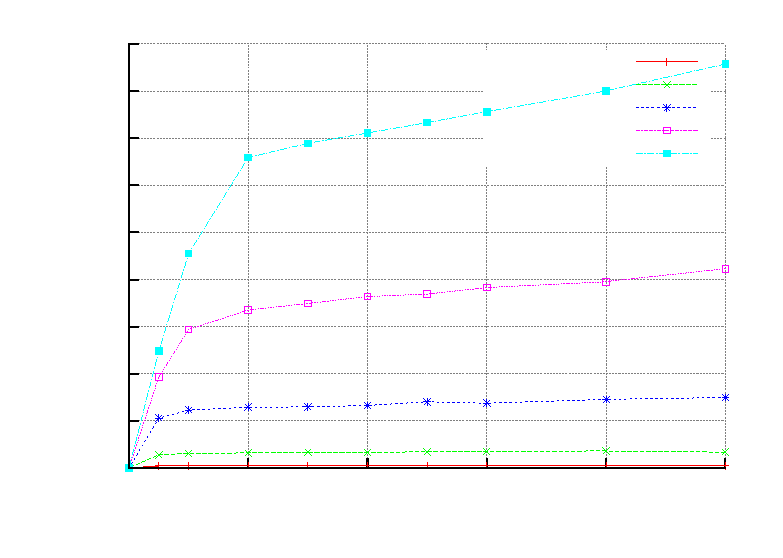
\includegraphics{graph}}%
    \gplfronttext
  \end{picture}%
\endgroup
}
  \caption{\label{fig:graph} Graph}
\end{figure}

\begin{table}[hbtp]
  \centering
  \begin{tabular}{c|ccc}
    $V_{TN}$ = \SI{2.11}{V} & $V_{DS}$ = \SI{0.5}{V} & $V_{DS}$ = \SI{1}{V} & $V_{DS}$ = \SI{1.5}{V} \\
    \hline
    $V_{GS}$ = \SI{2.91}{V} & & & 0.1078 \\
    $V_{GS}$ = \SI{2.71}{V} & & 0.0931 & \\
    $V_{GS}$ = \SI{2.51}{V} & 0.07688 & & \\
  \end{tabular}
  \caption{\label{tab:kn} $k_n'$}
\end{table}

\section{Conclusion}
\label{sec:conclusion}

\section{Equations}
\label{sec:equations}

% LaTeX sees blank lines as a start of another paragraph.  To avoid
% unnecessary vertical spaces between equations, and still visually
% separate in source, put a comment between them.
%
\begin{equation}
  \label{eq:transconduct}
  g_m = \frac{I_{D2}-I_{D1}}{V_{GS2}-V_{GS1}}
\end{equation}
%
\begin{equation}
  \label{eq:phys}
  \frac{k_n'}{2} \cdot \frac{W}{L} = \frac{I_{D1}}{(V_{GS1} - V_{TN})^2}
\end{equation}

\end{document}
